\subsection{理论依据}
\begin{align*}
    &span(E[I_p-Var(X|Y)]^2) \subseteq S_{Y|X}
\end{align*}
\subsection{样本计算流程}
\begin{enumerate}
    \item 将$X_1,\dots,X_n$标准化为$Z_1,\dots,Z_n$
    \item 将$[a,b]=[min{Y_i}_{i=1}^n,max{Y_i}_{i=1}^n]$划分为$k$个区间,得到$\widetilde{Y}_i$;由此计算$\bar{\mu}_i=\frac{1}{\#\{I_i\}}\sum_{Y_j\in I_i}Z_j$
    \item 计算条件方差估计量$\hat{\Sigma}_i=\sum_{i=1}^k\frac{1}{\#I_i}\sum_{Y_j\in I_i}(Z_j-\hat{\mu}_i)(Z_j-\hat{\mu}_i)^T$
    \item 计算协方差矩阵估计量
    \begin{align*}
        \widetilde{M}&=\sum_{i=1}^kE_n[I(Y\in I_i)] [I_{p\times p}-Var(Z|\widetilde{Y}=i)]^2 \\
        &=\sum_{i=1}^k\frac{\#\{I_i\}}{n}(I_{p\times p}-\hat{\Sigma}_i)^2
    \end{align*}
    \item 计算$\widetilde{M}$的前q个特征向量$u_1,\dots,u_n$,则对$S_{Y|X}$中向量的估计为$v_k=\hat{\Sigma}_{X}^{-1/2}u_k,k=1,\dots,q$
    
\end{enumerate}
在实际计算中,将$[Y_{(1),Y_(n)}]$划分为$10$个区间.
\subsection{线性回归模型}
设定样本量为1000,降维维数由$10-20$,判断其降维效果.
\begin{figure}[H]
    \centering
    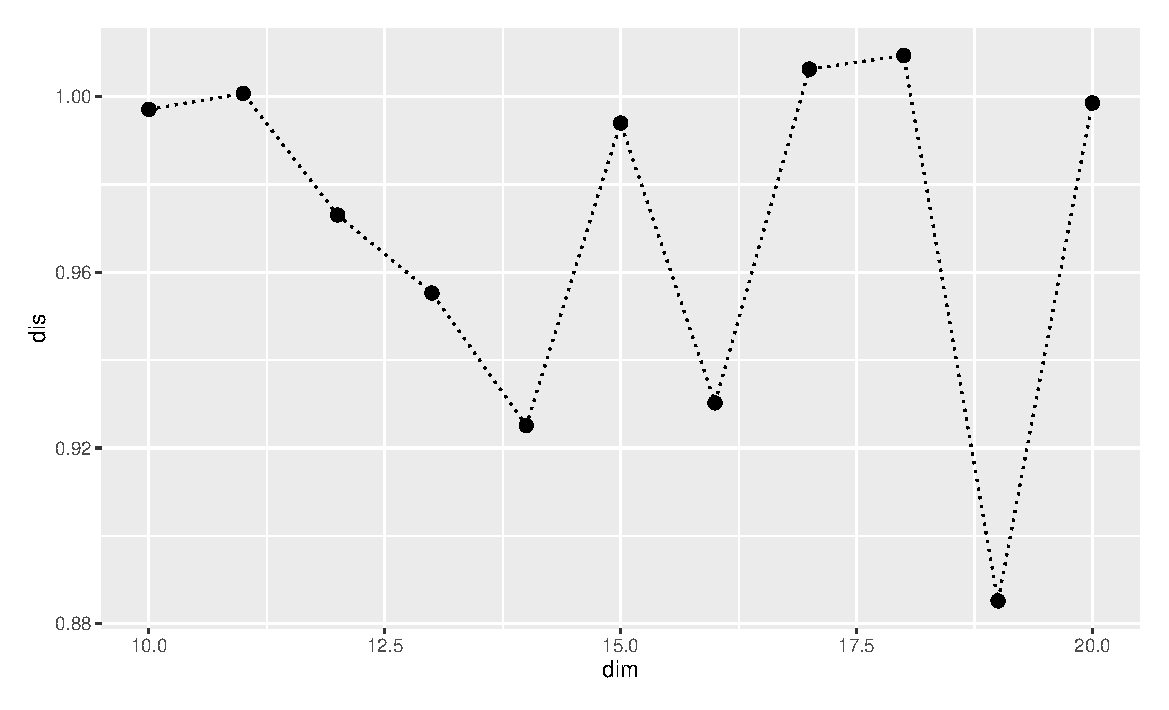
\includegraphics[width=0.8\textwidth]{image/norm_save.eps}
    \caption{线性回归下维度对降维效果的影响}
\end{figure}


\subsection{cos函数与sin函数生成的数据的降维计算}
按$y=\cos(2\beta_1^Tx)+\cos(\beta_2^Tx)+\varepsilon$,生成样本y。其中$\beta_1$是参数矩阵$\beta$的第一列向量,同理$\beta_2$,而$\varepsilon$服从均值为0,方差0.1的正态分布。对于sinh函数关系,我们按$y=\sin(2\beta_1^Tx)+\sin(\beta_2^Tx)+\varepsilon$,生成样本y。一维下就去掉$\beta_2^Tx$项。
\begin{figure}[H]
    \centering
    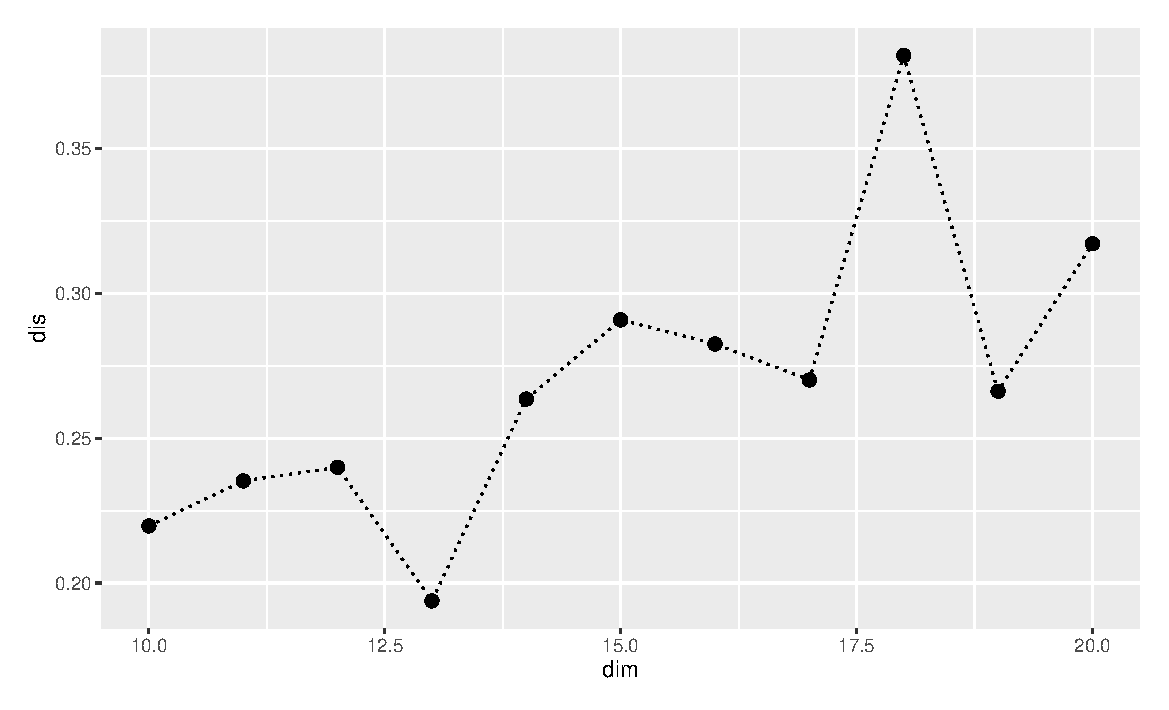
\includegraphics[width=0.8\textwidth]{image/cos_save.eps}
    \caption{cos函数生成的数据下维度对降维效果的影响(二维)}
\end{figure}

\begin{figure}[H]
    \centering
    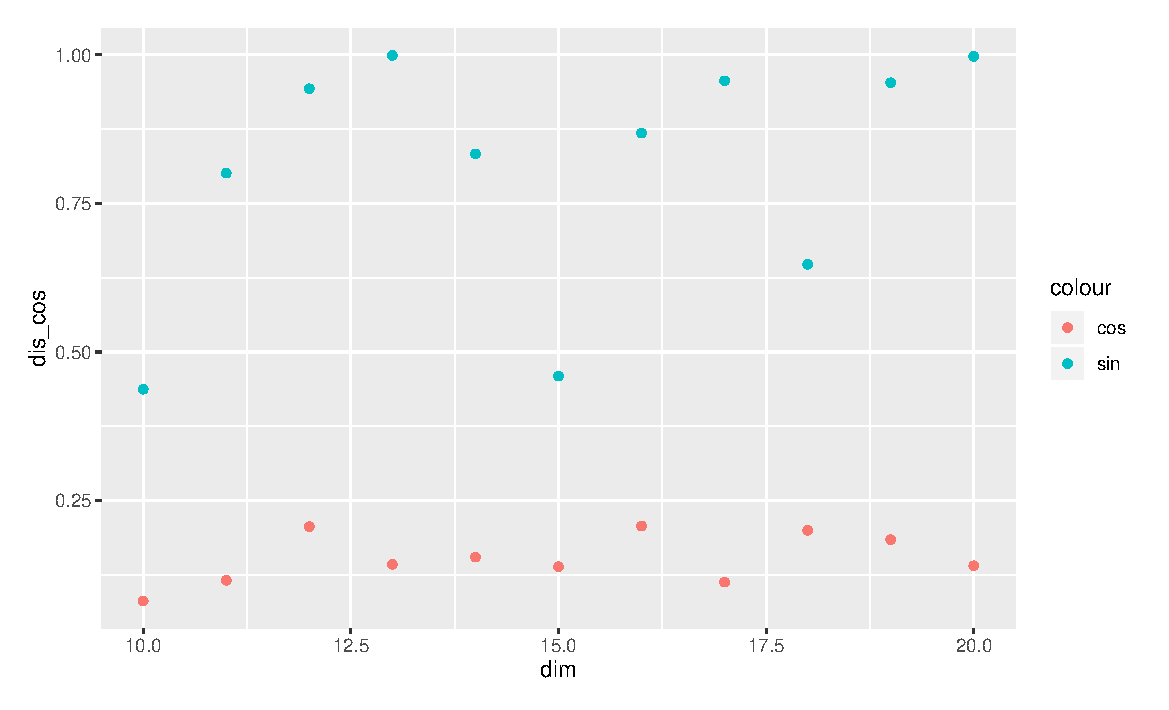
\includegraphics[width=0.8\textwidth]{image/compare_save_one.eps}
    \caption{cos函数与sin函数生成的数据下维度对降维效果的影响(一维)}
\end{figure}

而在将降维后维数分别设定为1,2,3,4,5时,其降维效果如图所示
\begin{figure}[H]
    \centering
    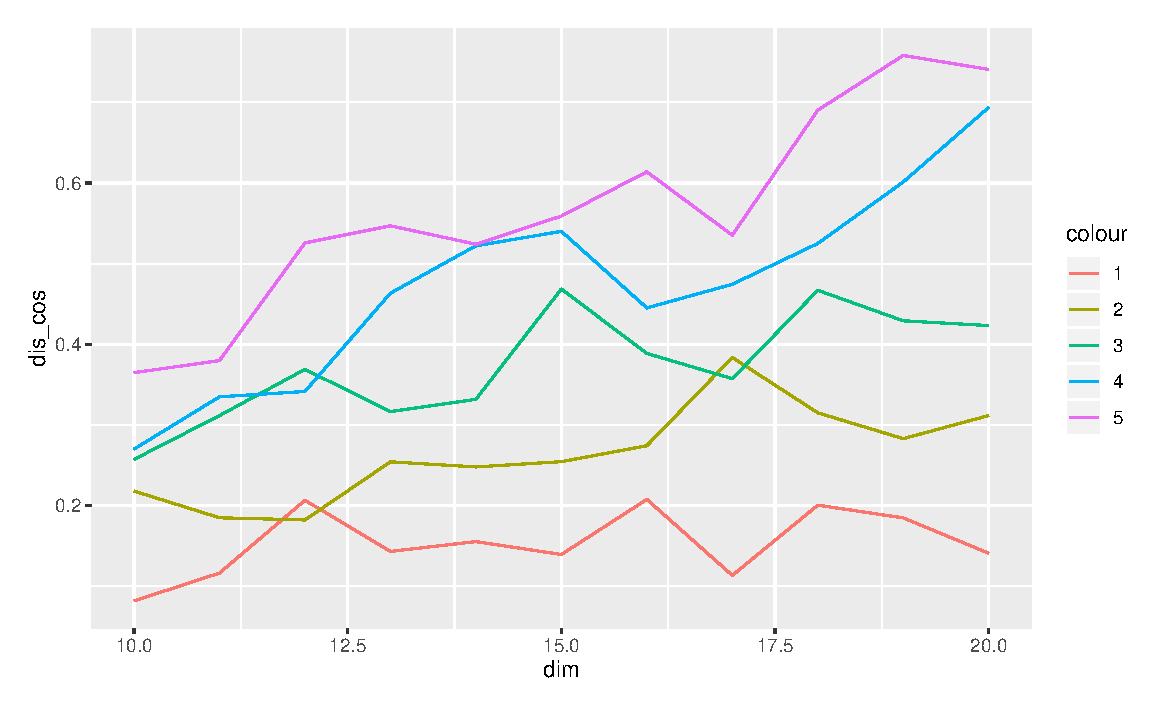
\includegraphics[width=0.8\textwidth]{image/compare_dim_save.eps}
    \caption{cos函数生成的数据下降维后维度对降维效果的影响}
\end{figure}

\subsection{总结}
从图像可以看出,样本量始终为1000的情况下,增大X的维数,估计空间与实际空间的差距呈上升趋势。
线性回归下,降维效果并不好,且从其波动性可以看出,模型结果首样本数据影响极大。
由cos函数生成的Y的数据降维效果较好,提高其生成函数实际空间的维数,可见虽维数上升,降维效果也有所下降。
而由sin函数生成的Y的数据降维效果则非常不好,与cos函数生成数据所做结果进行比较,我们可一推测SAVE的降维效果可能与Y与X之间函数关系的奇偶性有关。